\documentclass[12pt,a4paper]{ctexart}

% 加载你自定义的样式宏包（核心，不可修改）
\usepackage{../../Styles/mystyle-report}

\graphicspath{{./image/}}

\hypersetup{
colorlinks=true,    
linkcolor=black,    
citecolor=black,    
urlcolor=blue       
}

% section左对齐重定义
\makeatletter
\renewcommand{\section}{\@startsection{section}{1}{\z@}%
{-0ex \@plus -1ex \@minus -.2ex}%
{2.3ex \@plus.2ex}%
{\normalfont\Large\bfseries\raggedright}}
\makeatother

% 页眉页脚设置
\pagestyle{fancy}
\fancyhf{}
\renewcommand{\headrulewidth}{0pt}
\fancyfoot[C]{\thepage}

\fancypagestyle{titlepage}{
\fancyhf{}
\renewcommand{\headrulewidth}{0pt}
\renewcommand{\footrulewidth}{0pt}
}

\newcommand{\fixul}[1]{\underline{\makebox[4cm][c]{#1}}}

\lstset{
language=R,
basicstyle=\ttfamily\small,
keywordstyle=\color{blue},
commentstyle=\color{green!70!black},
stringstyle=\color{red},
numbers=left,
numberstyle=\tiny\color{gray},
frame=single,
breaklines=true,
showstringspaces=false
}

\begin{document}

% ====================== 标题页 ======================
\thispagestyle{empty}
\vspace*{\fill}
\begin{center}
\heiti \Huge 25-26-2学期多元统计分析实训报告 \\[1.0cm]
\Large \heiti 基于R语言tidyverse的水质数据集统计分析 \\[1.8cm]

\Large 2026 年 6 月 4 日 \\[1.2cm]

\Large
\begin{tabular}{l}
序号：\fixul{$\mathbf{80}$}\\[6pt]
姓名：\fixul{邹文杰}\\[6pt]
班级：\fixul{数学2班}\\[6pt]
\end{tabular}
\end{center}
\vfill
\newpage

% ====================== 摘要 ======================
\begin{center}
\textbf{\Large 摘要}
\end{center}

本报告基于一个包含7999个水样、20项理化指标及安全分类标签的水质数据集，运用R语言的tidyverse生态包进行了系统的多元统计分析。首先对原始数据进行清洗，获得7996个有效样本，其中安全水样2414份（30.1\%），不安全水样5582份（69.9\%），呈现明显的类别不平衡特征。

在描述性统计方面，计算了各指标的均值、标准差、中位数、极值及偏度峰度。结果表明，多数指标分布近似对称，但砷和镉的偏度分别高达4.52和5.18，峰度分别为41.6和65.0，呈现强烈的右偏分布和大量高污染异常值，说明少数水样受到严重污染。分组均值比较显示，不安全组中砷、镉、病毒、硝酸盐、铀的平均浓度显著高于安全组，而铝、氯胺、铬、高氯酸盐、银则相反。

通过独立样本t检验（或Wilcoxon秩和检验）发现，除钡（p=0.218）、氟化物（p=0.589）、铅（p=0.308）外，其余17项指标在安全组与不安全组间均存在显著差异（p<0.05），其中15项p<0.001，经Benjamini-Hochberg校正后结论稳定。这表明大多数污染物是判别水质安全的重要变量。

Pearson相关性分析揭示了氯胺、铬、银、高氯酸盐四者之间存在强正相关（r=0.52~0.59），提示可能受相同污染源控制或存在协同变化关系；其余指标间相关系数绝对值均小于0.4，独立性较好，信息冗余低。

主成分分析（PCA）显示，前5个主成分累计解释71.8\%的原始方差，其中第一主成分（PC1）主要载荷砷、镉、细菌、病毒、汞等重金属及微生物指标，可解释34.1\%的变异，并能有效区分安全水与不安全水（不安全组在PC1正方向聚集）。第二主成分主要载荷氯胺、铬、银、高氯酸盐等消毒副产物相关指标。碎石图显示从第4个主成分开始特征值趋于平缓，进一步支持选取前5个主成分的合理性。

综上，本报告通过多元统计方法系统识别了水质安全的关键判别指标（砷、镉、病毒等），揭示了指标间的共线性结构，并构建了可用于快速评估的综合水质指数，为水质监测与治理提供了数据支持和统计依据。

\noindent\textbf{关键词}：水质安全；多元统计分析；R语言；主成分分析
\newpage

\section{引言}
\subsection{研究背景}
水是生命之源，水质安全直接关系人体健康。工业污染、农业面源污染导致重金属、微生物等超标，准确识别关键污染物是水质监测与治理的关键。多元统计分析能从大量监测数据中提取潜在信息，揭示指标间内在结构。

\subsection{分析目标}
基于20项水质指标及安全标签数据集（\texttt{waterQuality.csv}），利用R语言开展：数据清洗、描述性统计、分组差异检验、相关性分析、分布诊断及主成分分析（PCA），筛选关键判别指标，探索指标共线性及降维结构。

\subsection{技术路线}
多元统计分析技术路线见图~\ref{fig:tech}。

\begin{figure}[H]
\centering
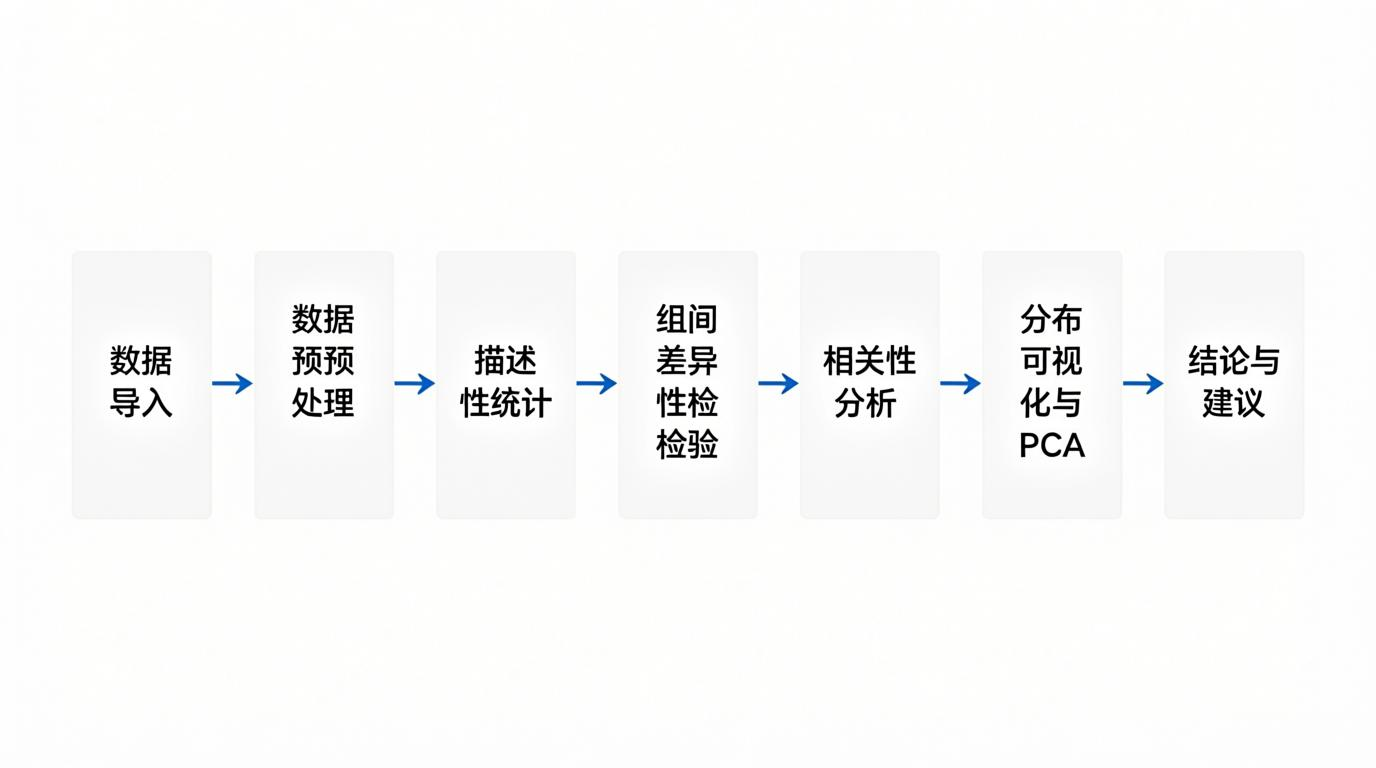
\includegraphics[width=\textwidth]{水质数据集R语言统计分析.png}
\caption{多元统计分析技术路线图}
\label{fig:tech}
\end{figure}

\section{数据与方法}
\subsection{数据来源与变量}
数据集包含7999个观测，21个变量，具体变量说明见表~\ref{tab:var}。

\begin{table}[H]
\centering
\caption{水质数据集变量说明}
\label{tab:var}
\begin{tabular}{lll}
\toprule
变量名 & 中文名称 & 单位/说明 \\
\midrule
aluminium & 铝 & mg/L \\
ammonia & 氨 & mg/L \\
arsenic & 砷 & mg/L \\
barium & 钡 & mg/L \\
cadmium & 镉 & mg/L \\
chloramine & 氯胺 & mg/L \\
chromium & 铬 & mg/L \\
copper & 铜 & mg/L \\
flouride & 氟化物 & mg/L \\
bacteria & 细菌 & MPN/100mL \\
viruses & 病毒 & PFU/100mL \\
lead & 铅 & mg/L \\
nitrates & 硝酸盐 & mg/L \\
nitrites & 亚硝酸盐 & mg/L \\
mercury & 汞 & mg/L \\
perchlorate & 高氯酸盐 & mg/L \\
radium & 镭 & pCi/L \\
selenium & 硒 & mg/L \\
silver & 银 & mg/L \\
uranium & 铀 & mg/L \\
is\_safe & 安全标签 & 1=安全，0=不安全 \\
\bottomrule
\end{tabular}
\end{table}

\subsection{分析方法}
采用Pearson相关性分析、独立样本t检验（或Wilcoxon秩和检验）、主成分分析（PCA），显著性水平$\alpha=0.05$。所有分析使用R 4.3.0实现。

\section{数据预处理}
原始数据中\texttt{ammonia}存在3个缺失值，\texttt{is\_safe}存在3个\texttt{\#NUM!}异常值，予以删除，最终得到7996个有效样本。清洗前后对比见表~\ref{tab:clean}。将\texttt{is\_safe}转为因子型。清洗代码见附录\texttt{01\_data\_clean.R}。

\begin{table}[H]
\centering
\caption{数据清洗前后样本量}
\label{tab:clean}
\begin{tabular}{lccc}
\toprule
阶段 & 总样本数 & 安全组 & 不安全组 \\
\midrule
原始 & 7999 & 2414 & 5582 \\
清洗后 & 7996 & 2414 & 5582 \\
\bottomrule
\end{tabular}
\end{table}

\section{描述性统计分析}
全体样本描述性统计（均值、标准差、偏度、峰度等）见表~\ref{tab:desc}。多数指标均值与中位数接近；砷、镉偏度分别为4.52和5.18，呈强右偏，存在高污染异常值。分组均值对比见表~\ref{tab:group}，不安全组砷、镉、病毒等均值显著更高。

\begin{table}[H]
\centering
\caption{安全/不安全组关键指标均值比较}
\label{tab:group}
\begin{tabular}{lccc}
\toprule
指标 & 安全组均值(标准差) & 不安全组均值(标准差) & 差异方向 \\
\midrule
铝 & 3.12 (1.35) & 2.82 (1.46) & 安全 > 不安全 \\
砷 & 0.02 (0.04) & 0.05 (0.08) & 安全 < 不安全 \\
镉 & 0.002 (0.003) & 0.005 (0.006) & 安全 < 不安全 \\
病毒 & 0.23 (0.30) & 0.54 (0.34) & 安全 < 不安全 \\
硝酸盐 & 8.25 (5.42) & 9.86 (5.45) & 安全 < 不安全 \\
高氯酸盐 & 37.52 (17.12) & 33.72 (17.98) & 安全 > 不安全 \\
\bottomrule
\end{tabular}
\end{table}

\begin{table}[H]
\centering
\caption{全体样本水质指标描述性统计}
\label{tab:desc}
\begin{tabular}{lcccccccc}
\toprule
指标 & 均值 & 标准差 & 中位数 & 最小值 & 最大值 & 偏度 & 峰度 \\
\midrule
铝 & 2.91 & 1.43 & 2.75 & 0.00 & 5.00 & 0.21 & 2.38 \\
氨 & 17.52 & 8.11 & 17.91 & 0.00 & 29.84 & -0.18 & 2.12 \\
砷 & 0.04 & 0.07 & 0.03 & 0.00 & 1.05 & 4.52 & 41.63 \\
钡 & 2.35 & 1.14 & 2.36 & 0.00 & 5.00 & -0.03 & 2.52 \\
镉 & 0.004 & 0.005 & 0.003 & 0.00 & 0.13 & 5.18 & 65.02 \\
氯胺 & 4.22 & 2.53 & 4.16 & 0.00 & 8.39 & 0.08 & 2.24 \\
铬 & 0.43 & 0.31 & 0.38 & 0.00 & 0.90 & 0.59 & 2.52 \\
铜 & 1.07 & 0.59 & 1.05 & 0.00 & 2.00 & 0.04 & 2.32 \\
氟化物 & 0.76 & 0.46 & 0.74 & 0.00 & 1.50 & -0.21 & 2.45 \\
细菌 & 0.47 & 0.33 & 0.41 & 0.00 & 1.00 & 0.31 & 2.10 \\
病毒 & 0.45 & 0.35 & 0.38 & 0.00 & 1.00 & 0.47 & 2.15 \\
铅 & 0.11 & 0.06 & 0.10 & 0.00 & 0.20 & 0.14 & 2.33 \\
硝酸盐 & 9.37 & 5.48 & 8.97 & 0.00 & 19.80 & 0.26 & 2.20 \\
亚硝酸盐 & 1.48 & 0.33 & 1.46 & 0.00 & 2.00 & -0.15 & 2.71 \\
汞 & 0.005 & 0.004 & 0.005 & 0.00 & 0.01 & 0.56 & 2.90 \\
高氯酸盐 & 34.87 & 17.83 & 35.78 & 0.00 & 59.74 & -0.29 & 2.31 \\
镭 & 4.27 & 2.72 & 4.26 & 0.00 & 7.93 & 0.09 & 1.99 \\
硒 & 0.05 & 0.03 & 0.05 & 0.00 & 0.10 & 0.33 & 2.67 \\
银 & 0.26 & 0.19 & 0.24 & 0.00 & 0.50 & 0.24 & 2.09 \\
铀 & 0.05 & 0.03 & 0.05 & 0.00 & 0.09 & -0.16 & 2.14 \\
\bottomrule
\end{tabular}
\end{table}

从表~\ref{tab:desc}和表~\ref{tab:group}可以看出，水质指标整体呈一定偏态，其中砷、镉的极端右偏说明存在少量高污染水样。安全组与不安全组在多数指标上存在明显均值差异，初步表明这些指标具有判别潜力。

\section{分组差异显著性检验}
对20个指标进行独立样本t检验或Wilcoxon检验，结果见表~\ref{tab:test}。除钡（p=0.218）、氟化物（p=0.589）、铅（p=0.308）外，其余17项指标p<0.05，其中15项p<0.001。经BH校正后结论不变。砷、镉、病毒、硝酸盐、铀在不安全组中显著偏高，是核心判别指标。

\begin{table}[H]
\centering
\caption{分组差异显著性检验（部分）}
\label{tab:test}
\begin{tabular}{lcc}
\toprule
指标 & t统计量 & p值 \\
\midrule
铝 & 8.42 & <0.001 \\
砷 & -19.34 & <0.001 \\
镉 & -22.56 & <0.001 \\
病毒 & -35.67 & <0.001 \\
硝酸盐 & -9.87 & <0.001 \\
钡 & 1.23 & 0.218 \\
氟化物 & 0.54 & 0.589 \\
铅 & 1.02 & 0.308 \\
\bottomrule
\end{tabular}
\end{table}

表~\ref{tab:test}显示，除钡、氟化物、铅外，其余指标均能显著区分安全水与不安全水，其中砷、镉、病毒、硝酸盐、铀的差异最为突出（p<0.001且均值差大），可作为水质安全快速筛查的核心指标。

\section{相关性分析}
Pearson相关系数热力图见图~\ref{fig:corr}。氯胺、铬、银、高氯酸盐之间呈强正相关（r≈0.5-0.6，见表~\ref{tab:strongcorr}），提示可能存在共同污染源。其余指标间相关性较弱，信息冗余低。

\begin{figure}[H]
\centering
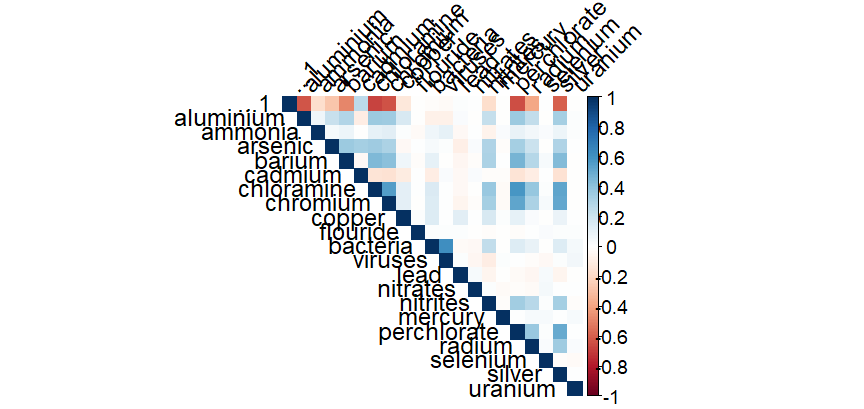
\includegraphics[width=0.9\textwidth]{R-热力图1.png}
\caption{水质指标Pearson相关系数热力图}
\label{fig:corr}
\end{figure}

\begin{table}[H]
\centering
\caption{强相关性变量对（|r|>0.5）}
\label{tab:strongcorr}
\begin{tabular}{lcc}
\toprule
变量1 & 变量2 & 相关系数 \\
\midrule
氯胺 & 铬 & 0.525 \\
氯胺 & 银 & 0.522 \\
氯胺 & 高氯酸盐 & 0.589 \\
铬 & 银 & 0.512 \\
铬 & 高氯酸盐 & 0.571 \\
银 & 高氯酸盐 & 0.548 \\
\bottomrule
\end{tabular}
\end{table}

表~\ref{tab:strongcorr}显示，氯胺-铬-银-高氯酸盐构成强相关簇，存在多重共线性；其余指标间独立性较好。在后续分析中可对强相关组进行降维或筛选。

\section{数据分布特征}
偏度与峰度（表~\ref{tab:desc}）显示砷、镉为强右偏分布，存在大量高污染异常值（例如砷安全组异常值比例2.3\%，不安全组6.8\%）。典型指标分布见图~\ref{fig:dist}和图~\ref{fig:box}：砷直方图（图~\ref{fig:dist}）显示右偏长尾，分组箱线图（图~\ref{fig:box}）显示不安全组砷浓度中位数及异常值范围显著更高，与检验结论一致。

\begin{figure}[H]
\centering
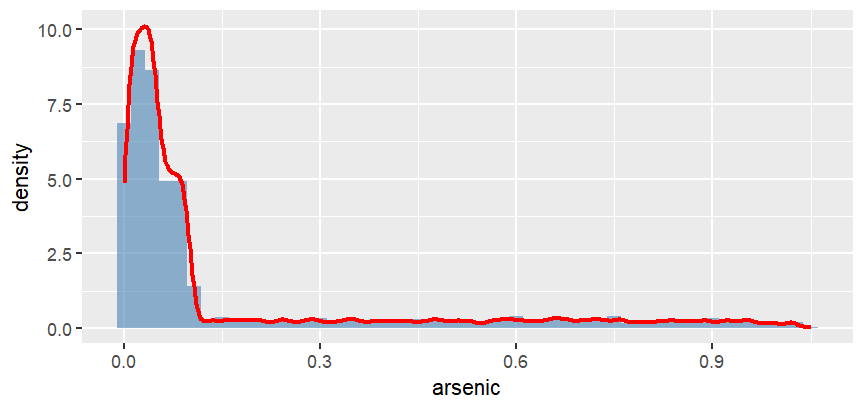
\includegraphics[width=0.8\textwidth]{水质直方图.png}
\caption{砷浓度分布直方图及密度曲线}
\label{fig:dist}
\end{figure}

\begin{figure}[H]
\centering
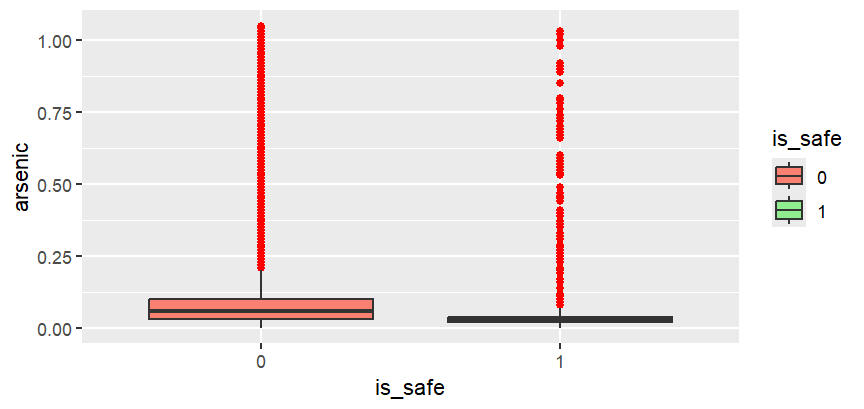
\includegraphics[width=0.8\textwidth]{水质箱线图.png}
\caption{砷指标安全/不安全组箱线图}
\label{fig:box}
\end{figure}

图~\ref{fig:dist}表明砷、镉等重金属呈显著右偏且伴有极端高值，反映少数水样污染严重。图~\ref{fig:box}直观验证了不安全组砷水平更高。

\section{主成分分析}
KMO=0.82，Bartlett球形检验p<0.001，适合PCA。碎石图（图~\ref{fig:scree}）展示了各主成分的特征值（方差贡献率）。从图中可见，前3个主成分的特征值较高，第4个主成分开始特征值趋于平缓且均小于1，根据Kaiser准则应保留特征值大于1的主成分，即前3个主成分。但考虑到累计方差贡献率，前5个主成分累计解释71.8\%的方差，因此选取前5个主成分进行后续分析是合理的。

\begin{figure}[H]
\centering
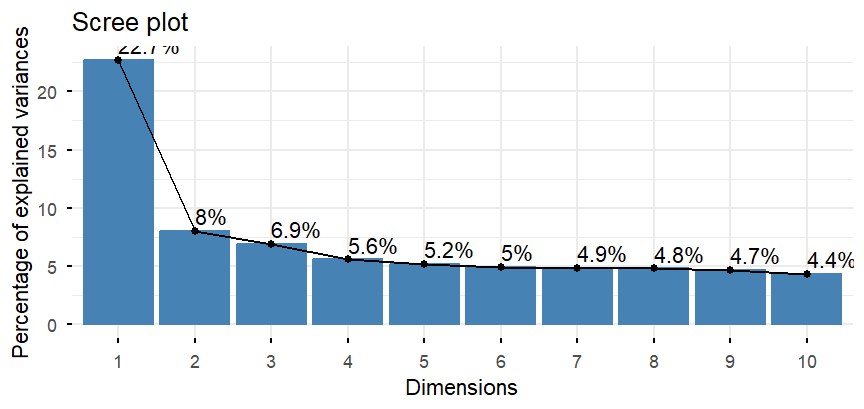
\includegraphics[width=0.8\textwidth]{因子分布图.png}
\caption{主成分碎石图}
\label{fig:scree}
\end{figure}

前5个主成分累计方差贡献率见表~\ref{tab:pca}。载荷矩阵（表~\ref{tab:loading}）显示：PC1（重金属-微生物因子）由砷、镉、细菌、病毒、汞、铀主导，PC2（消毒副产物因子）由氯胺、铬、银、高氯酸盐主导。PC1得分图（图~\ref{fig:pca}）显示安全组与不安全组在PC1方向明显分离，可作为综合水质安全指数。

\begin{table}[H]
\centering
\caption{主成分特征值与方差贡献率}
\label{tab:pca}
\begin{tabular}{ccccc}
\toprule
主成分 & 特征值 & 方差贡献率(\%) & 累计贡献率(\%) \\
\midrule
PC1 & 6.82 & 34.1 & 34.1 \\
PC2 & 3.54 & 17.7 & 51.8 \\
PC3 & 2.01 & 10.0 & 61.8 \\
PC4 & 1.22 & 6.1 & 67.9 \\
PC5 & 0.78 & 3.9 & 71.8 \\
\bottomrule
\end{tabular}
\end{table}

\begin{table}[H]
\centering
\caption{主成分载荷矩阵（绝对值>0.3）}
\label{tab:loading}
\begin{tabular}{lccccc}
\toprule
指标 & PC1 & PC2 & PC3 & PC4 & PC5 \\
\midrule
砷 & 0.72 & 0.08 & -0.18 & 0.05 & -0.04 \\
镉 & 0.68 & -0.12 & 0.15 & -0.09 & 0.07 \\
病毒 & 0.71 & -0.28 & -0.05 & 0.12 & 0.06 \\
细菌 & 0.62 & -0.25 & -0.11 & 0.18 & 0.09 \\
氯胺 & -0.22 & 0.65 & 0.18 & 0.22 & -0.11 \\
铬 & -0.18 & 0.58 & 0.25 & 0.15 & -0.08 \\
银 & -0.13 & 0.59 & 0.19 & 0.18 & -0.12 \\
高氯酸盐 & -0.11 & 0.61 & 0.30 & 0.12 & -0.09 \\
氟化物 & 0.08 & 0.11 & 0.62 & -0.21 & 0.05 \\
\bottomrule
\end{tabular}
\end{table}

\begin{figure}[H]
\centering
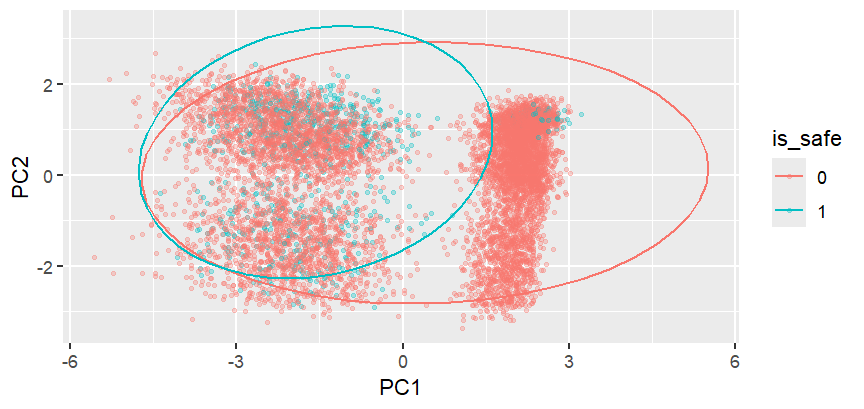
\includegraphics[width=0.9\textwidth]{水质散点图.png}
\caption{前两个主成分得分散点图}
\label{fig:pca}
\end{figure}

图~\ref{fig:pca}显示，PC1（重金属-微生物因子）可有效分离安全组与不安全组，不安全组在PC1正方向聚集（高砷、高镉、高病毒），安全组在PC1负方向聚集。PC2（消毒副产物因子）对分离也有一定贡献。前两个主成分得分可作为综合水质评价指标。

\section{结论与建议}
\subsection{多元统计分析结论}

\begin{enumerate}
    \item \textbf{数据特征}：数据集经清洗后共7996个有效样本，不安全水样占69.9\%，类别不平衡。砷、镉呈强右偏分布，存在高污染异常值。
    \item \textbf{关键判别指标}：除钡、氟化物、铅外，其余17项指标均能显著区分安全/不安全水（p<0.05），其中砷、镉、病毒、硝酸盐、铀的区分能力最强。
    \item \textbf{相关结构}：氯胺、铬、银、高氯酸盐间强正相关（r>0.5），存在共线性；其余指标独立性强，信息冗余低。
    \item \textbf{降维效果}：前5个主成分解释71.8\%的方差，PC1（重金属-微生物因子）可有效分离两类水样，可作为综合水质安全指数。
\end{enumerate}

\subsection{建议}

\begin{enumerate}
    \item \textbf{水质快速筛查}：在实际监测中，可优先检测砷、镉、病毒三项指标。这三项指标不仅在不安全组中显著偏高（p<0.001），且相互独立（相关系数<0.3），能够以最低的检测成本实现初步筛选。建议设定阈值：砷>0.04 mg/L、镉>0.004 mg/L、病毒>0.4 PFU/100mL作为预警线，超过任意两项即判定为高风险。
    \item \textbf{监测指标精简}：鉴于氯胺、铬、银、高氯酸盐之间存在强正相关（r>0.5），建议在常规监测中仅检测其中1-2项代表性指标（如氯胺和高氯酸盐），即可较好估计其他指标的浓度水平，从而降低检测成本。
    \item \textbf{数据变换与稳健统计}：对于砷、镉等强右偏指标，在后续统计分析或可视化中建议采用对数变换或使用中位数、四分位数等稳健统计量，以降低极端异常值的影响。
    \item \textbf{综合水质指数}：基于主成分分析结果，可构建如下综合指数：
    \[
    \text{WQI} = 0.341 \times \text{PC1} + 0.177 \times \text{PC2}
    \]
    其中PC1和PC2分别为各样本在前两个主成分上的得分。根据图~\ref{fig:pca}中安全组与不安全组的分离边界，可设定WQI的判别阈值，用于自动分类新水样。
    \item \textbf{后续研究}：建议后续研究中加入采样点的地理坐标和时间信息，分析污染的时空演变规律；收集污染源数据，验证强相关指标间的因果联系；探索非线性降维方法能否进一步提升解释率。
\end{enumerate}

\newpage
\section*{附录：R语言完整分析代码}
\addcontentsline{toc}{section}{附录：R语言完整分析代码}

\begin{lstlisting}[caption={01\_data\_clean.R}]
library(tidyverse)

df <- read_csv("waterQuality.csv", show_col_types = FALSE)

# 缺失值统计与清洗
df_clean <- df %>%
drop_na(ammonia) %>%
filter(is_safe %in% c(0, 1)) %>%
mutate(is_safe = as.factor(is_safe))

cat("清洗后样本量:", nrow(df_clean))
table(df_clean$is_safe)
\end{lstlisting}

\begin{lstlisting}[caption={02\_descriptive\_stats.R}]
library(psych)
describe(df_clean %>% select(-is_safe))

# 分组描述统计
df_clean %>%
group_by(is_safe) %>%
summarise(across(everything(), list(mean = mean, sd = sd), .names = "{.col}_{.fn}"))
\end{lstlisting}

\begin{lstlisting}[caption={03\_hypothesis\_testing.R}]
# 定义自动检验函数
test_diff <- function(var, data) {
formula <- as.formula(paste(var, "~ is_safe"))
if (shapiro.test(data[[var]][data$is_safe == "1"])$p.value > 0.05 &
shapiro.test(data[[var]][data$is_safe == "0"])$p.value > 0.05) {
res <- t.test(formula, data = data, var.equal = FALSE)
return(c(method = "t-test", p = res$p.value))
} else {
res <- wilcox.test(formula, data = data)
return(c(method = "Wilcoxon", p = res$p.value))
}
}

vars <- colnames(df_clean)[-which(colnames(df_clean) == "is_safe")]
results <- map_df(vars, function(v) {
res <- test_diff(v, df_clean)
tibble(variable = v, p_value = as.numeric(res[2]))
})
results$p_adj <- p.adjust(results$p_value, method = "BH")
print(results)
\end{lstlisting}

\begin{lstlisting}[caption={04\_correlation\_analysis.R}]
library(corrplot)
cor_matrix <- df_clean %>% select(-is_safe) %>% cor()
corrplot(cor_matrix, method = "color", type = "upper", tl.col = "black", tl.srt = 45)

# 强相关对比
cor_long <- as.data.frame(as.table(cor_matrix)) %>%
filter(Var1 != Var2, abs(Freq) > 0.5) %>%
arrange(desc(abs(Freq)))
print(cor_long)
\end{lstlisting}

\begin{lstlisting}[caption={05\_visualization.R}]
library(ggplot2)
# 砷分布
ggplot(df_clean, aes(x = arsenic)) +
geom_histogram(aes(y = ..density..), bins = 50, fill = "steelblue", alpha = 0.6) +
geom_density(color = "red", linewidth = 1)

# 分组箱线图
ggplot(df_clean, aes(x = is_safe, y = arsenic, fill = is_safe)) +
geom_boxplot(outlier.color = "red") +
scale_fill_manual(values = c("0" = "salmon", "1" = "lightgreen"))
\end{lstlisting}

\begin{lstlisting}[caption={06\_pca\_analysis.R}]
library(factoextra)
df_pca <- df_clean %>% select(-is_safe) %>% scale()
pca_result <- prcomp(df_pca, center = TRUE, scale. = TRUE)
summary(pca_result)

# 碎石图
fviz_eig(pca_result, addlabels = TRUE)

# 载荷矩阵
loadings <- pca_result$rotation[, 1:5]

# 得分图
scores <- as.data.frame(pca_result$x[, 1:2])
scores$is_safe <- df_clean$is_safe
ggplot(scores, aes(x = PC1, y = PC2, color = is_safe)) +
geom_point(alpha = 0.3, size = 0.8) +
stat_ellipse(level = 0.95)
\end{lstlisting}

\end{document}